% ==============================================================================
% Modelo para Especificação de Projeto de Software
% Prof. Vítor E. Silva Souza - NEMO/UFES :: DI/UFES :: PPGI/UFES
%
% Baseado em abtex2-modelo-trabalho-academico.tex, v-1.9.2 laurocesar
% Copyright 2012-2014 by abnTeX2 group at http://abntex2.googlecode.com/ 
%
% This work may be distributed and/or modified under the conditions of the LaTeX 
% Project Public License, either version 1.3 of this license or (at your option) 
% any later version. The latest version of this license is in
% http://www.latex-project.org/lppl.txt.
%
% IMPORTANTE:
% Instruções encontram-se espalhadas pelo documento. Para facilitar sua leitura,
% tais instruções são precedidas por (*) -- utilize a função localizar do seu
% editor para passar por todas elas.
% ==============================================================================

% Usa o estilo abntex2, configurando detalhes de formatação e hifenização.
\documentclass[
	12pt,				
	oneside,		
	a4paper,			
	english,			% Idioma adicional para hifenização.
	french,				% Idioma adicional para hifenização.
	spanish,			% Idioma adicional para hifenização.
	brazil				% O último idioma é o principal do documento.
	]{abntex2}


%%% Importação de pacotes. %%%

% Conserta o erro "No room for a new \count". 
% O comando \reserveinserts deve ser comentado ou não, dependendo da versão do LaTeX.
\usepackage{etex}
%\reserveinserts{28}

% Usa a fonte Latin Modern.
\usepackage{lmodern}

% Seleção de códigos de fonte.
\usepackage[T1]{fontenc}

% Codificação do documento em Unicode.
\usepackage[utf8]{inputenc}

% Usado pela ficha catalográfica.
\usepackage{lastpage}

% Indenta o primeiro parágrafo de cada seção.
\usepackage{indentfirst}

% Controle das cores.
\usepackage[usenames,dvipsnames]{xcolor}

% Inclusão de gráficos.
\usepackage{graphicx}

% Melhor controle de leiaute de tabelas.
\usepackage{tabularx}
\usepackage{colortbl}
\usepackage{longtable}
\usepackage{pdflscape}

% Inclusão de páginas em PDF diretamente no documento (para uso nos apêndices).
\usepackage{pdfpages}

% Para melhorias de justificação.
\usepackage{microtype}

% Citações padrão ABNT.
\usepackage[brazilian,hyperpageref]{backref}
\usepackage[alf]{abntex2cite}	
\renewcommand{\backrefpagesname}{Citado na(s) página(s):~}		% Usado sem a opção hyperpageref de backref.
\renewcommand{\backref}{}										% Texto padrão antes do número das páginas.
\renewcommand*{\backrefalt}[4]{									% Define os textos da citação.
	\ifcase #1
		Nenhuma citação no texto.
	\or
		Citado na página #2.
	\else
		Citado #1 vezes nas páginas #2.
	\fi}

% \rm is deprecated and should not be used in a LaTeX2e document
% http://tex.stackexchange.com/questions/151897/always-textrm-never-rm-a-counterexample
\renewcommand{\rm}{\textrm}

% Inclusão de símbolos não padrão.
\usepackage{amssymb}
\usepackage{eurosym}

% Para utilizar \eqref para referenciar equações.
\usepackage{amsmath}

% Permite mostrar figuras muito largas em modo paisagem com \begin{sidewaysfigure} ao invés de \begin{figure}.
\usepackage{rotating}

% Permite customizar listas enumeradas/com marcadores.
\usepackage{enumitem}

% Permite inserir hiperlinks com \url{}.
\usepackage{bigfoot}
\usepackage{hyperref}

% Permite usar o comando \hl{} para evidenciar texto com fundo amarelo. Útil para chamar atenção a itens a fazer.
\usepackage{soulutf8}

% Colorinlistoftodos package: to insert colored comments so authors can collaborate on the content.
% (*) Indicar o nome do aluno e substituir o nome do professor se for o caso.
\usepackage[colorinlistoftodos, textwidth=20mm, textsize=footnotesize]{todonotes}
\newcommand{\aluno}[1]{\todo[author=\textbf{Aluno},color=green!30,caption={},inline]{#1}}
\newcommand{\vitor}[1]{\todo[author=\textbf{Vítor},color=red!30,caption={},inline]{#1}}

% Permite inserir espaço em branco condicional (incluído no texto final só se necessário) em macros.
\usepackage{xspace}

% Permite incluir listagens de código com o comando \lstinputlisting{}.
\usepackage{listings}
\usepackage{caption}
\DeclareCaptionFont{white}{\color{white}}
\DeclareCaptionFormat{listing}{\colorbox{gray}{\parbox{\textwidth}{#1#2#3}}}
\captionsetup[lstlisting]{format=listing,labelfont=white,textfont=white}
\renewcommand{\lstlistingname}{Listagem}
\definecolor{mygray}{rgb}{0.5,0.5,0.5}
\lstset{
	basicstyle=\scriptsize,
	breaklines=true,
	numbers=left,
	numbersep=5pt,
	numberstyle=\tiny\color{mygray}, 
	rulecolor=\color{black},
	showstringspaces=false,
	tabsize=2,
    inputencoding=utf8,
    extendedchars=true,
    literate=%
    {é}{{\'{e}}}1
    {è}{{\`{e}}}1
    {ê}{{\^{e}}}1
    {ë}{{\¨{e}}}1
    {É}{{\'{E}}}1
    {Ê}{{\^{E}}}1
    {û}{{\^{u}}}1
    {ù}{{\`{u}}}1
    {â}{{\^{a}}}1
    {à}{{\`{a}}}1
    {á}{{\'{a}}}1
    {ã}{{\~{a}}}1
    {Á}{{\'{A}}}1
    {Â}{{\^{A}}}1
    {Ã}{{\~{A}}}1
    {ç}{{\c{c}}}1
    {Ç}{{\c{C}}}1
    {õ}{{\~{o}}}1
    {ó}{{\'{o}}}1
    {ô}{{\^{o}}}1
    {Õ}{{\~{O}}}1
    {Ó}{{\'{O}}}1
    {Ô}{{\^{O}}}1
    {î}{{\^{i}}}1
    {Î}{{\^{I}}}1
    {í}{{\'{i}}}1
    {Í}{{\~{Í}}}1
}




%%% Definição de variáveis. %%%
% (*) Substituir os textos abaixo com as informações apropriadas.
\titulo{English For All Time}
\autor{Matheus De Oliveira Lima}
\local{Vitória, ES}
\data{\the\year}
\instituicao{
	Universidade Federal do Espírito Santo -- UFES
	\par
	Centro Tecnológico
	\par
	Departamento de Informática}
\newcommand{\subtitulo}{Documento de Projeto de Sistema}
\newcommand{\versao}{1.0}

% Define a capa.
\renewcommand{\imprimircapa}{%
	\begin{capa}%
		\center
		
		{\ABNTEXchapterfont\large\subtitulo{}}
		\vfill
		\begin{center}
			\ABNTEXchapterfont\bfseries\LARGE\imprimirtitulo
		\end{center}
		
		\vfill
		\large\imprimirlocal
		\linebreak
		\large\imprimirdata
		\vspace*{1cm}
	\end{capa}
}

% Macros específicas do trabalho.
% (*) Inclua aqui termos que são utilizados muitas vezes e que demandam formatação especial.
% Exemplo: Java com TM (trademark) em superscript.
% Use sempre \xspace para que o LaTeX inclua espaço em branco após a macro somente quando necessário.
\newcommand{\java}{Java\texttrademark\xspace}




%%% Configurações finais de aparência. %%%

% Altera o aspecto de algumas cores.
\definecolor{blue}{RGB}{41,5,195}
\definecolor{lightgray}{gray}{0.9}

% Informações do PDF.
\makeatletter
\hypersetup{
	pdftitle={\@title}, 
	pdfauthor={\@author},
	pdfsubject={\imprimirpreambulo},
	pdfcreator={LaTeX with abnTeX2},
	pdfkeywords={abnt}{latex}{abntex}{abntex2}{trabalho acadêmico}, 
	colorlinks=true,				% Colore os links (ao invés de usar caixas).
	linkcolor=blue,					% Cor dos links.
	citecolor=blue,					% Cor dos links na bibliografia.
	filecolor=magenta,				% Cor dos links de arquivo.
	urlcolor=blue,					% Cor das URLs.
	bookmarksdepth=4
}
\makeatother

% Espaçamentos entre linhas e parágrafos.
\setlength{\parindent}{1.3cm}
\setlength{\parskip}{0.2cm}



%%% Páginas iniciais do documento: capa, folha de rosto, ficha, resumo, tabelas, etc. %%%

% Compila o índice.
\makeindex

% Inicia o documento.
\begin{document}

% Retira espaço extra obsoleto entre as frases.
\frenchspacing

% Inclui o brasão da UFES.
\begin{figure}[h]
  \centering
  
\includegraphics[scale=0.055]{brasao.jpg}
  \label{ppts3}
\end{figure} 

% Capa do trabalho.
\imprimircapa


% (*) Incluir linhas no registro de alterações a cada nova versão.
\begin{center}
	{\large\bfseries Registro de Alterações:}
	
	\vspace{0.5cm}
	\begin{tabular}{|c|p{45mm}|c|p{60mm}|} \hline
		
		\textbf{Versão} & \textbf{Responsável} & \textbf{Data}  & \textbf{Alterações} \\ \hline   
		
		1.0  & Matheus De Oliveira & 27/05/2025 & Versão inicial. \\\hline 
	\end{tabular}
\end{center}
\newpage



%%% Início da parte de conteúdo do documento. %%%
% Marca o início dos elementos textuais.
\textual

% Inclusão dos capítulos como seções (sem quebra de página).
\begingroup
\let\clearpage\relax

% ==============================================================================
% Projeto de Sistema - Matheus De Oliveira Lima
% Capítulo 1 - Introdução
% ==============================================================================
\chapter{Introdução}
\label{sec-intro}
\vspace{-1cm}

Este documento apresenta o projeto (\textit{design}) do sistema \emph{\imprimirtitulo}. 

É um plataforma de ensino de inglês onde o professor-administrador tem controle total: ele pode cadastrar seus alunos e adicionar/criar cursos diretamente no sistema, organizando-os em módulos com vídeos (via links do YouTube não listados), materiais em PDF e exercícios. A plataforma oferece um painel intuitivo para o dono gerenciar tanto os usuários quanto os conteúdos publicados, permitindo atualizações rápidas e personalizadas, sem depender de terceiros. E para os alunos eles terão uma página com todos os conteúdos publicados pelo professor.

%\vitor{Completar o parágrafo acima com uma breve descrição do sistema.}

Além desta introdução, este documento está organizado da seguinte forma: 
a Seção~\ref{sec-plataforma} apresenta a plataforma de software utilizada na implementação do sistema;
a Seção~\ref{sec-arquitetura} apresenta a arquitetura de software; por fim, 
a Seção~\ref{sec-frameweb} apresenta os modelos FrameWeb que descrevem os componentes da arquitetura.


\vspace*{1.5cm}

% ==============================================================================
% Projeto de Sistema - Matheus De Oliveira Lima
% Capítulo 2 - Plataforma de Desenvolvimento
% ==============================================================================
\chapter{Plataforma de Desenvolvimento}
\label{sec-plataforma}
\vspace{-1cm}


%\vitor{Esta seção deve apresentar a plataforma de implementação a ser adotada para o desenvolvimento do sistema, incluindo: linguagem de programação, mecanismo de persistência de dados e componentes ou \textit{frameworks} a serem usados. As tabelas abaixo trazem exemplos (defasados) que devem ser adaptados para o contexto do seu projeto.}


%=======================================================================================================
%			Tabela de Plataforma de Desenvolvimento e Tecnologias Utilizadas
%=======================================================================================================

Na Tabela~\ref{tabela-plataforma} são listadas as tecnologias utilizadas no desenvolvimento da ferramenta, bem como o propósito de sua utilização.

\begin{footnotesize}
\begin{longtable}{|p{1.8cm}|c|p{5cm}|p{6.3cm}|}
	\caption{Plataforma de Desenvolvimento e Tecnologias Utilizadas.}	
	\label{tabela-plataforma}\\\hline

	\rowcolor{lightgray}
	\textbf{Tecnologia} & \textbf{Versão} & \textbf{Descrição} & \textbf{Propósito} \\\hline 
	\endfirsthead
	\hline
	\rowcolor{lightgray}
	\textbf{Tecnologia} & \textbf{Versão} & \textbf{Descrição} & \textbf{Propósito} \\\hline 
	\endhead
		
	React.js & 18+ & Biblioteca JavaScript para interfaces dinâmicas & Frontend responsivo para alunos e admin \\ \hline
	
	TypeScript & 5.x & Superset tipado de JavaScript & Frontend responsivo para alunos e admin \\ \hline
	
	Spring Boot & 3.2.x (Java 17) & Framework backend Java & API RESTful segura e escalável \\ \hline
	
	Spring Web MVC & 6.1.x & Módulo para construção de APIs REST & Rotas HTTP e serialização JSON \\ \hline
	
	Spring Security & 6.1.x & Autenticação e autorização & Controle de acesso (JWT) \\ \hline
	
	Spring Data JPA & 3.1.x & Persistência com Hibernate & Operações de banco de dados (PostgreSQL) \\ \hline
	
	PostgreSQL & 15+ & Banco de dados relacional & Armazenar usuários, cursos e progresso \\ \hline
	
	jjwt & 0.12.x & Biblioteca para JWT & Geração/validação de tokens \\ \hline
	
	Lombok & 1.18.x & Redução de boilerplate em classes Java & Getters/Setters automáticos \\ \hline
	
	Hibernate Validator & 8.0.x & Validação de dados em DTOs & Validar entradas de API (ex.: @Email, @NotBlank) \\ \hline
	
	React Router & 6.x & Roteamento no frontend & Navegação entre páginas \\ \hline
	
	Axios & 1.x & Cliente HTTP para frontend & Consumir API do backend \\ \hline
	
	Material-UI & 5.x & Biblioteca de componentes UI & Design consistente e responsivo \\ \hline
	
\end{longtable}
\end{footnotesize}






%=======================================================================================================
%			Tabela de Softwares de Apoio ao Desenvolvimento do Projeto
%=======================================================================================================

Na Tabela~\ref{tabela-software} vemos os softwares que apoiaram o desenvolvimento de documentos e também do código fonte.

\begin{footnotesize}
\begin{longtable}{|p{2.5cm}|c|p{5cm}|p{5.5cm}|}
	\caption{Softwares de Apoio ao Desenvolvimento do Projeto}	
	\label{tabela-software}\\\hline
	
	\rowcolor{lightgray}
	\textbf{Tecnologia} & \textbf{Versão} & \textbf{Descrição} & \textbf{Propósito} \\\hline 
	\endfirsthead
	\hline
	\rowcolor{lightgray}
	\textbf{Tecnologia} & \textbf{Versão} & \textbf{Descrição} & \textbf{Propósito} \\\hline 
	\endhead
	
	PgAdmin 4 & 7.x+ & Interface gráfica para PostgreSQL & Gerenciar visualmente o banco de dados \\\hline
	
	IntelliJ IDEA & 2023.2+ & IDE para Java/Spring Boot & Desenvolvimento backend com debug integrado \\\hline 
	
	VS Code & 1.80+ & Editor para React/TypeScript & Codificação do frontend com extensões úteis \\\hline
	
	Postman & 10+ & Teste de APIs & Validar endpoints do Spring Boot \\\hline 
	
	Git & 2.40+ & Controle de versão & Gerenciar colaboração no código \\\hline 
	 
	FrameWeb Editor & 1.0 & Ferramenta CASE do método FrameWeb. & Criação dos modelos de Entidades, Aplicação, Persistência e Navegação. \\\hline

	TeX Live  & 2018 & Implementação do \LaTeX & Documentação do projeto arquitetural do sistema. \\\hline       
	
	TeXstudio & 4.8.7 & Editor de LaTeX. &  Escrita da documentação do sistema, sendo usado o \textit{template} \textit{abnTeX}.\footnote{\url{http://www.abntex.net.br}.} \\\hline    
	
	Apache Maven & 3.5 & Ferramenta de gerência/construção de projetos de software. & Obtenção e integração das dependências do projeto. \\\hline
\end{longtable}
\end{footnotesize}

\vspace*{1.5cm}

\chapter{Requisitos Não Funcionais}
\label{sec-rnfs}
\vspace{-1cm}

A Tabela~\ref{tabela-rnfs} apresenta a especificação dos requisitos não funcionais identificados no Documento de Especificação de Requisitos, os quais foram considerados condutores da arquitetura.

% Contador para IDs de Requisitos Não Funcionais.
% Substitua rnf-definir-label dentro dos \label{} abaixo por IDs do seu projeto.
\newcounter{rnfcount}
\renewcommand*\thernfcount{RNF-\arabic{rnfcount}}
\newcommand*\RNF{\refstepcounter{rnfcount}\thernfcount}
\setcounter{rnfcount}{0}

\begin{footnotesize}
\begin{longtable}{|r|p{13cm}|}
	\caption{Especificação de Requisitos Não Funcionais.}
	\label{tabela-rnfs}\\\hline
	
	\multicolumn{2}{|p{\dimexpr\linewidth-2\tabcolsep-2\arrayrulewidth}|}{\cellcolor{lightgray}\RNF\label{rnf-definir-label01} -- sentença descrevendo o RNF, conforme Documento de Especificação de Requisitos.}\\\hline
	
	Categoria: & \hl{Possíveis valores: Interoperabilidade, Segurança, Usabilidade, Eficiência, Confiabilidade, Disponibilidade, Manutenibilidade, Portabilidade.} \\\hline
	
	\parbox[t]{2cm}{\raggedleft Tática /\\Tratamento:} & \hl{Apontar a tática a ser usada e algum detalhe, quando pertinente sobre como essa tática será aplicada no contexto do projeto.} \\\hline
	
	Medida: & \hl{Medida a ser usada para estabelecer objetivamente um critério de aceitação para o atendimento do RNF.} \\\hline
	
	\parbox[t]{2cm}{\raggedleft Critério de\\Aceitação:} & \hl{Descrição do critério de aceitação. Deve permitir avaliar objetivamente se o RNF foi satisfeito ou não.} \\\hline
	
	% Linha em branco.
	\multicolumn{2}{c}{}\\\hline
	
	\multicolumn{2}{|p{\dimexpr\linewidth-2\tabcolsep-2\arrayrulewidth}|}{\cellcolor{lightgray}\RNF\label{rnf-definir-label02} -- sentença descrevendo o RNF, conforme Documento de Especificação de Requisitos.}\\\hline
	
	Categoria: & \hl{Possíveis valores: Interoperabilidade, Segurança, Usabilidade, Eficiência, Confiabilidade, Disponibilidade, Manutenibilidade, Portabilidade.} \\\hline
	
	\parbox[t]{2cm}{\raggedleft Tática /\\Tratamento:} & \hl{Apontar a tática a ser usada e algum detalhe, quando pertinente sobre como essa tática será aplicada no contexto do projeto.} \\\hline
	
	Medida: & \hl{Medida a ser usada para estabelecer objetivamente um critério de aceitação para o atendimento do RNF.} \\\hline
	
	\parbox[t]{2cm}{\raggedleft Critério de\\Aceitação:} & \hl{Descrição do critério de aceitação. Deve permitir avaliar objetivamente se o RNF foi satisfeito ou não.} \\\hline

	% Linha em branco.
	\multicolumn{2}{c}{}\\\hline
	
	\multicolumn{2}{|p{\dimexpr\linewidth-2\tabcolsep-2\arrayrulewidth}|}{\cellcolor{lightgray}\RNF\label{rnf-definir-label03} -- Segurança}\\\hline
	
	Categoria: & \hl{Segurança.} \\\hline
	
	\parbox[t]{2cm}{\raggedleft Tática /\\Tratamento:} & \hl {Uso de JWT (jjwt) com chave HMAC-SHA256 para autenticação.} \\\hline
	
	Medida: & \hl{100\% dos endpoints protegidos por token JWT válido.} \\\hline
	
	\parbox[t]{2cm}{\raggedleft Critério de\\Aceitação:} & \hl{Testes automatizados verificam acesso negado a endpoints sem token.} \\\hline
	
\end{longtable}
\end{footnotesize}

\vspace*{1.5cm}


\chapter{Arquitetura de Software}
\label{sec-arquitetura}
\vspace{-1cm}

A Figura~\ref{figura-arquitetura} mostra a arquitetura do sistema \emph{\imprimirtitulo}. Ela é baseada em uma combinação dos estilos arquitetônicos Camadas e Partições.

\begin{figure}[h]
	\centering
	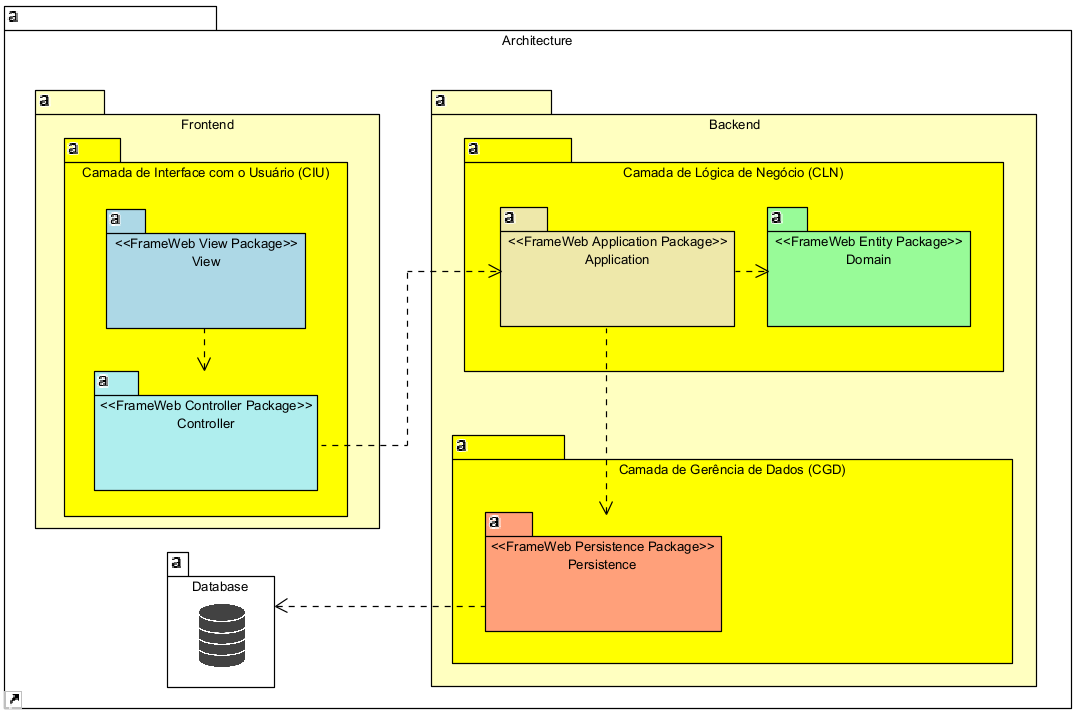
\includegraphics[width=0.8\textwidth]{figuras/architecture_novo.png}
	\caption{Arquitetura de Software.}
	\label{figura-arquitetura}
\end{figure}

A arquitetura do sistema é estruturada em três camadas principais, cada uma com responsabilidades distintas e bem definidas, conforme ilustrado na Figura ~\ref{figura-arquitetura}.

\section{Camada de Interface com o Usuário (CIU)}

Localizada no \textbf{Frontend}, essa camada é responsável pela interação com os usuários, exibindo dados e capturando ações externas. Ela adota o padrão \textbf{MVCS (Model-View-Controller-Service)} e está dividida em dois pacotes principais:

\begin{itemize}
	\item \textbf{View (\texttt{<<FrameWeb View Package>>})}: Contém os elementos da camada de apresentação, como páginas web, folhas de estilo, imagens e scripts do lado cliente.
	\item \textbf{Controller (\texttt{<<FrameWeb Controller Package>>})}: Coordena a interação entre a visão e os serviços da aplicação localizados na camada de lógica de negócio (CLN). A dependência entre os componentes é unidirecional: a \textit{view} depende do \textit{controller}, e este depende da lógica de aplicação.
\end{itemize}

\section{Camada de Lógica de Negócio (CLN)}

Localizada no \textbf{Backend}, essa camada implementa as regras de negócio do sistema. Ela segue o padrão \textbf{Camada de Serviço}, conforme definido por Fowler (2002), e é composta por dois pacotes:

\begin{itemize}
	\item \textbf{Application (\texttt{<<FrameWeb Application Package>>})}: Contém as classes responsáveis pela orquestração das funcionalidades do sistema, utilizando objetos de domínio e interagindo com a camada de persistência.
	\item \textbf{Domain (\texttt{<<FrameWeb Entity Package>>})}: Reúne as classes que representam os elementos centrais do domínio do problema. Tais entidades são manipuladas pela \textit{application} para a implementação das regras de negócio.
\end{itemize}

\section{Camada de Gerência de Dados (CGD)}

Também localizada no \textbf{Backend}, essa camada é responsável pela persistência dos dados e segue o padrão \textbf{Data Access Object (DAO)}. Contém o seguinte pacote:

\begin{itemize}
	\item \textbf{Persistence (\texttt{<<FrameWeb Persistence Package>>})}: Inclui as classes responsáveis pelas operações de acesso a dados, realizando mapeamento objeto-relacional (ORM) para persistir as entidades do domínio no banco de dados relacional.
\end{itemize}

\section{Integração entre as Camadas}

\begin{itemize}
	\item A \textbf{View} se comunica com o \textbf{Controller}.
	\item O \textbf{Controller} interage com a camada \textbf{Application}.
	\item A \textbf{Application} manipula entidades do \textbf{Domain} e utiliza a camada \textbf{Persistence} para realizar a persistência dos dados.
	\item A \textbf{Persistence} acessa diretamente o \textbf{banco de dados relacional}.
\end{itemize}

%\vitor{Substituir a Figura~\ref{figura-arquitetura} pelo diagrama UML da arquitetura do seu projeto e descrevê-la no texto. Caso use alguma arquitetura clássica, incluir referência bibliográfica com BibTeX (ex.:~\cite{fowler:book02}).}

\vspace*{1.5cm}


\chapter{Modelagem FrameWeb}
\label{sec-frameweb}
\vspace{-1cm}

\emph{\imprimirtitulo} é um sistema Web cuja arquitetura utiliza \textit{frameworks} comuns no desenvolvimento para esta plataforma. Desta forma, o sistema pode ser modelado utilizando a abordagem FrameWeb~\cite{souza-celebratingfalbo20}.

A Tabela~\ref{tabela-frameworks} indica os \textit{frameworks} presentes na arquitetura do sistema que se encaixam em cada uma das categorias de \textit{frameworks} que FrameWeb dá suporte. Em seguida, os modelos FrameWeb são apresentados para cada camada da arquitetura.

%\vitor{Substituir os valores da segunda coluna da Tabela~\ref{tabela-frameworks} pelos \textit{frameworks} utilizados no seu projeto. Remover o \hl{fundo amarelo}.}


\begin{footnotesize}
	\begin{longtable}{|c|c|}
		\caption{\textit{Frameworks} da arquitetura do sistema separados por categoria.}
		\label{tabela-frameworks}\\\hline
		
		\rowcolor{lightgray}
		\textbf{Categoria de \textit{Framework}} & \textbf{\textit{Framework} Utilizado} \\\hline 
		\endfirsthead
		\hline
		\rowcolor{lightgray}
		\textbf{Categoria de \textit{Framework}} & \textbf{\textit{Framework} Utilizado} \\\hline 
		\endhead

		Controlador Frontal & Spring MVC \\\hline

		Injeção de Dependências & Spring Framework \\\hline

		Mapeamento Objeto/Relacional & Spring Data JPA \\\hline

		Segurança & Spring Security \\\hline
	\end{longtable}
\end{footnotesize}




\section{Camada de Negócio}
\label{sec-frameweb-negocio}

%\vitor{Apresentar os modelos de entidades e de aplicação do FrameWeb.}

A figura~\ref{domain} mostra o projeto da Camada de Negócio (pacote \textsf{domain}) do sistema.

\begin{figure}[h]
	\centering
	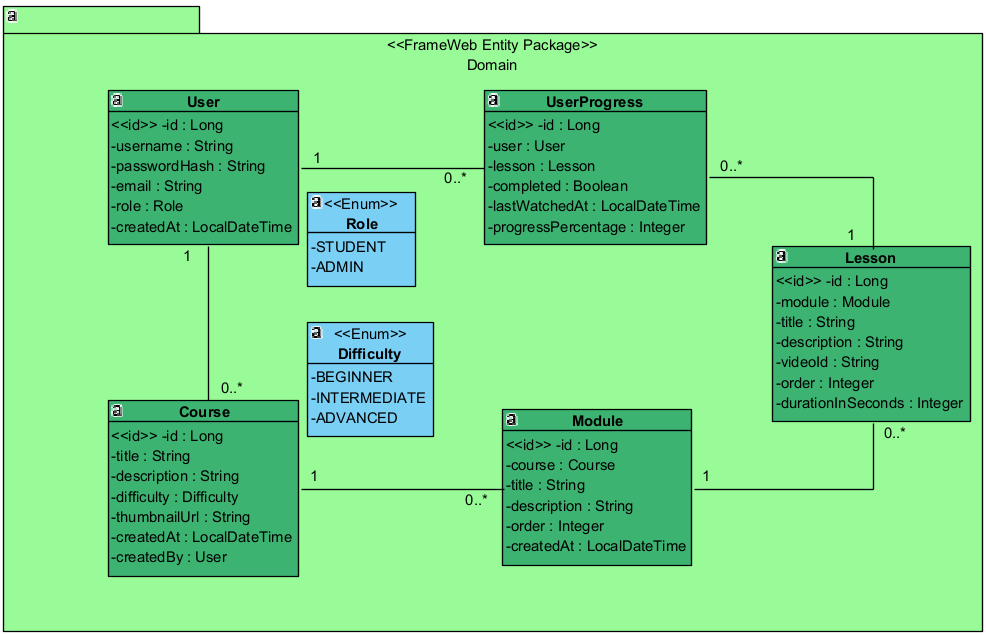
\includegraphics[width=0.8\textwidth]{figuras/domain.png}
	\caption{Projeto da Camada de Negócio (\textsf{domain})}
	\label{domain}
\end{figure}

Dentro do pacote \textsf{domain}, existem as entidades em verde escuro que são usadas como base das regras de negócio e da persistência de dados; enquanto as classes em azul claro, são tipos enumerados que representam classificações de usuário dentro do sistema (\textsf{Role}) e identificação da dificuldade de um curso (\textsf{Difficulty}).

\begin{figure}[h]
	\centering
	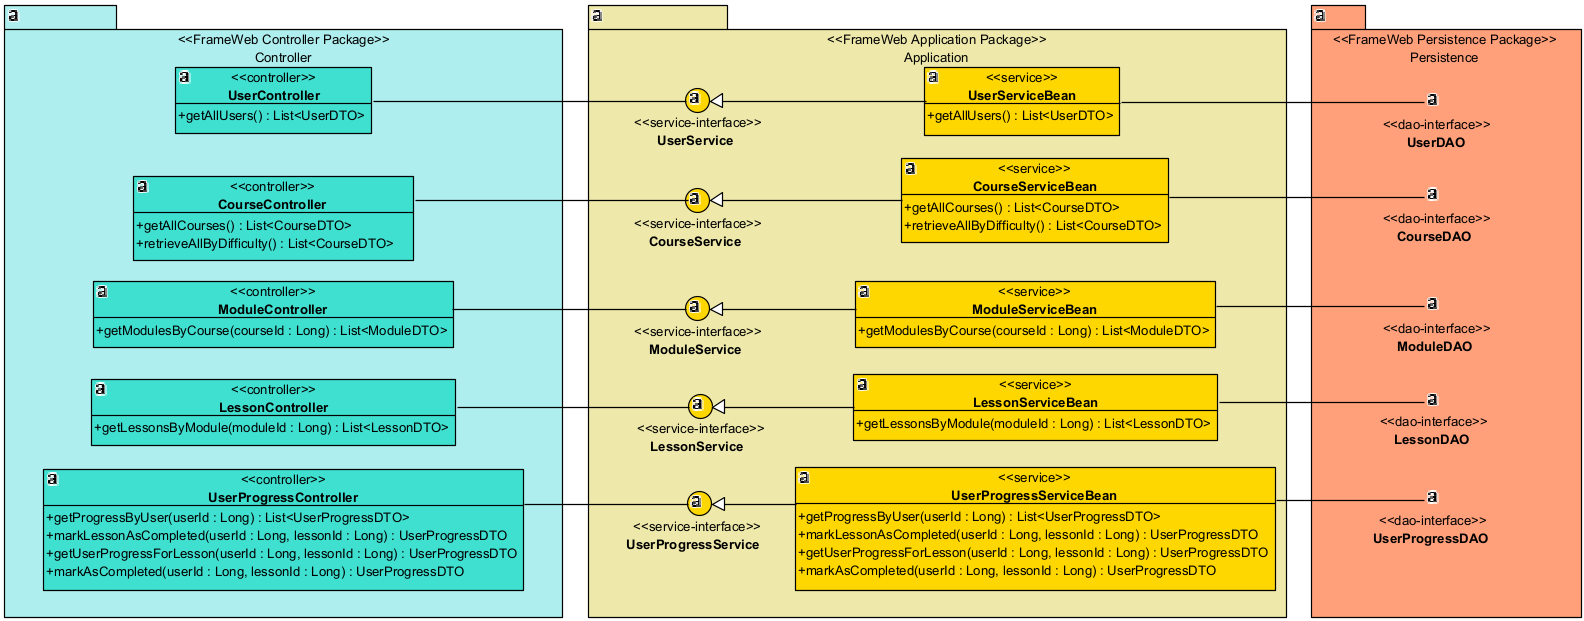
\includegraphics[width=0.8\textwidth]{figuras/application.png}
	\caption{Projeto da Camada de Negócio (\textsf{application})}
	\label{application}
\end{figure}

A arquitetura apresentada na Figura~\ref{application} ilustra a integração entre os pacotes Controller, Application e Persistence, os quais, em conjunto, viabilizam o retorno ao frontend dos resultados decorrentes da aplicação das regras de negócio solicitadas.

Vale destacar que, por se tratarem de operações básicas comuns a todas as entidades, as classes responsáveis pelas operações CRUD (\textsf{create, read, update e delete}) não foram explicitamente representadas na figura. Além disso, embora os métodos dos \textsf{controllers} retornem os dados encapsulados em objetos do tipo \textsf{ResponseEntity}, esse detalhe também foi omitido na representação para manter o diagrama mais conciso e focado na estrutura geral do fluxo de dados e responsabilidades.

\section{Camada de Acesso a Dados}
\label{sec-frameweb-dados}

%\vitor{Apresentar os modelos de persistência do FrameWeb.}

A figura~\ref{persistence} mostra o projeto da Camada de Acesso a Dados (pacote \textsf{persistence}) do sistema.

\begin{figure}[h]
	\centering
	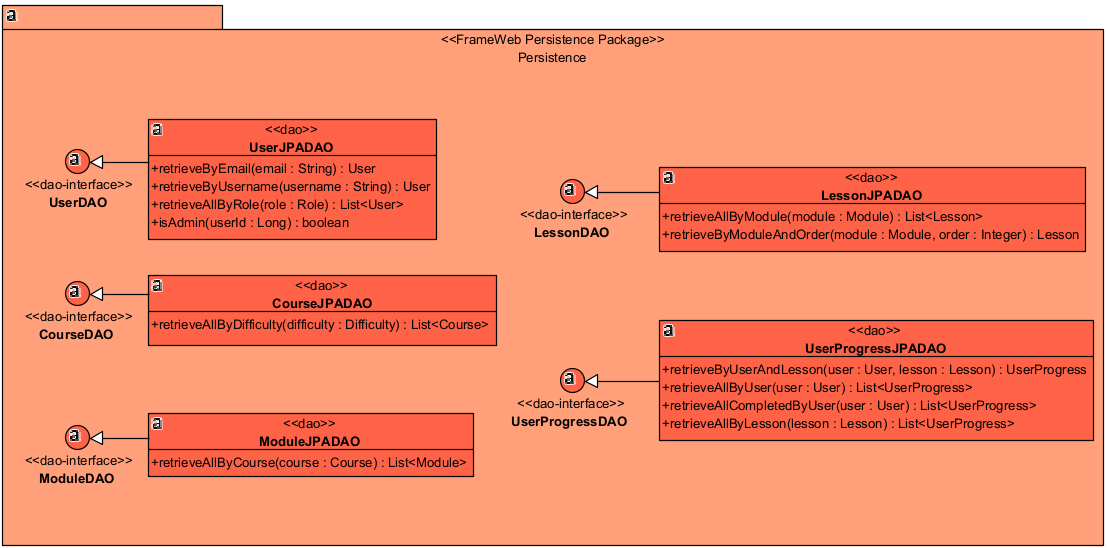
\includegraphics[width=0.8\textwidth]{figuras/persistence.png}
	\caption{Projeto de Acesso a Dados (\textsf{persistence})}
	\label{persistence}
\end{figure}

Nessa camada, como estará sendo utilizado o \textsf{Spring Data JPA}, por padrão ele já tem as buscas como create, read, update e delete (CRUD) das entidades básicas. Então, dentro de cada JPADAO do pacote \textsf{persistence} terão seus métodos personalizados que variam de acordo com a necessidade de acesso a dados do backend para aplicar suas regras de negócio que vão ser passadas ao \textsf{frontend}.

Enquanto o \textsf{Spring Data JPA}, há os métodos personalizados que fazem:

\begin{itemize}
	\item \textbf{UserJPADAO}: autenticação, recuperação de senha, validação de cadastro, cadastro/validação de nomes únicos, listar todos os alunos ou administradores e garantir que o usuário está acessando a área administrativa.
	
	\item \textbf{CourseJPADAO}: visualizar detalhes de um curso, vincular módulos a um curso, filtrar cursos por dificuldade.
	
	\item \textbf{ModuleJPADAO}: listar todos os módulos de um curso quando o aluno entra no curso.
	
	\item \textbf{LessonJPADAO}: listar as aulas dentro de um módulo, buscar uma aula específica em uma ordem (ex: próxima aula).
	
	\item \textbf{UserProgressJPADAO}: verificar se o aluno já completou a lição, listar progresso completo do aluno (quais aulas ele já viu), exibir o número de lições concluídas e estatísticas da aula: quantos alunos viram aquela lição.
\end{itemize}

\section{Camada de Apresentação}
\label{sec-frameweb-apresentacao}

\vitor{Apresentar os modelos de navegação do FrameWeb.}

\begin{figure}[h]
	\centering
	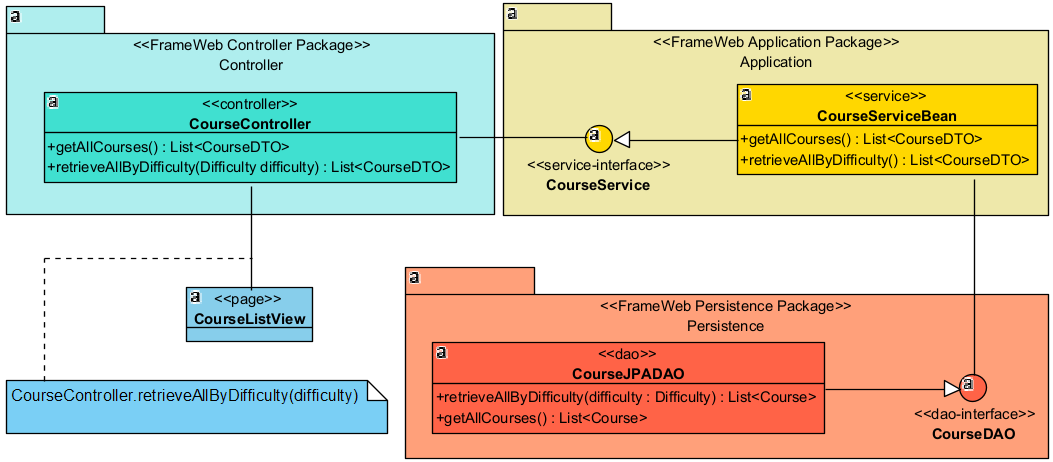
\includegraphics[width=0.8\textwidth]{figuras/visualizarCursos.png}
	\caption{Modelo de Navegação (\textsf{Visualizar Cursos})}
	\label{visualizarCursos}
\end{figure}

A imagem~\ref{visualizarCursos} representa a arquitetura da funcionalidade de consulta de cursos disponíveis em uma aplicação web estruturada segundo o padrão \textsf{FrameWeb}.

A operação é iniciada na camada de controle, com o método \textsf{retrieveAllByDifficulty(difficulty)} do \textsf{CourseController}, responsável por receber a requisição da interface de usuário, mais especificamente da página \textsf{CourseListView}, e encaminhá-la para a camada de aplicação. Nessa camada, o \textsf{CourseServiceBean}, implementando a interface \textsf{CourseService}, executa a lógica de negócio associada à recuperação de cursos conforme o nível de dificuldade selecionado, garantindo a aplicação das regras do domínio.

O \textsf{service} então delega a consulta à camada de persistência, onde o \textsf{CourseJPADAO}, implementação da interface \textsf{CourseDAO}, executa o método \textsf{retrieveAllByDifficulty}, realizando a busca no banco de dados e retornando uma lista de entidades \textsf{Course}. Além disso, a arquitetura contempla também o método \textsf{getAllCourses}, que possibilita a listagem completa dos cursos sem filtragem, percorrendo a mesma estrutura de camadas.

\begin{figure}[h]
	\centering
	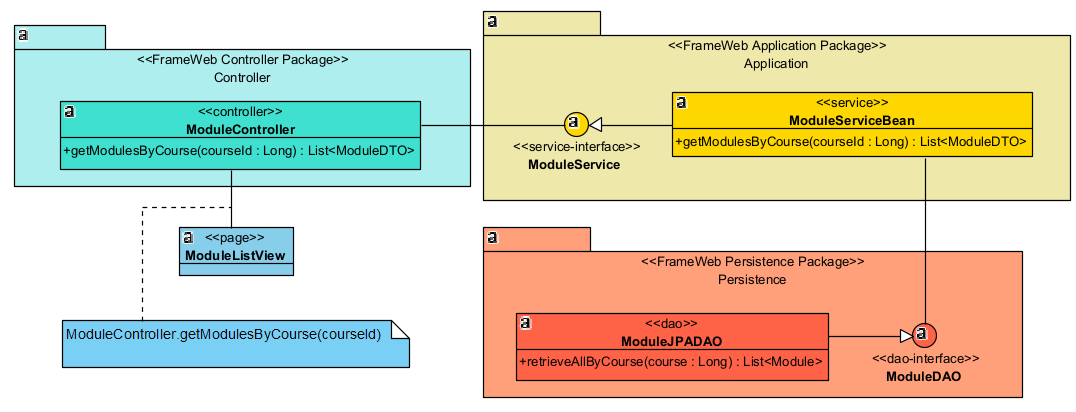
\includegraphics[width=0.8\textwidth]{figuras/visualizarModulosCurso.png}
	\caption{Modelo de Navegação (\textsf{Visualizar Módulos de um Curso})}
	\label{visualizarModulosCurso}
\end{figure}

A imagem~\ref{visualizarModulosCurso} representa a arquitetura da funcionalidade de consulta dos módulos de um curso em uma aplicação web estruturada segundo o padrão \textsf{FrameWeb}.

A operação é iniciada na camada de controle, com o método \textsf{getModulesByCourse(courseId)} do \textsf{ModuleController}, responsável por receber a requisição da interface de usuário, mais especificamente da página \textsf{ModuleListView}, e encaminhá-la para a camada de aplicação. Nessa camada, o \textsf{ModuleServiceBean}, implementando a interface \textsf{ModuleService}, executa a lógica de negócio associada à recuperação dos módulos pertencentes ao curso identificado pelo parâmetro \textsf{courseId}, garantindo a aplicação das regras do domínio.

O \textsf{service} então delega a consulta à camada de persistência, onde o \textsf{ModuleJPADAO}, implementação da interface \textsf{ModuleDAO}, executa o método \textsf{retrieveAllByCourse}, realizando a busca no banco de dados e retornando uma lista de entidades \textsf{Module}.

\begin{figure}[h]
	\centering
	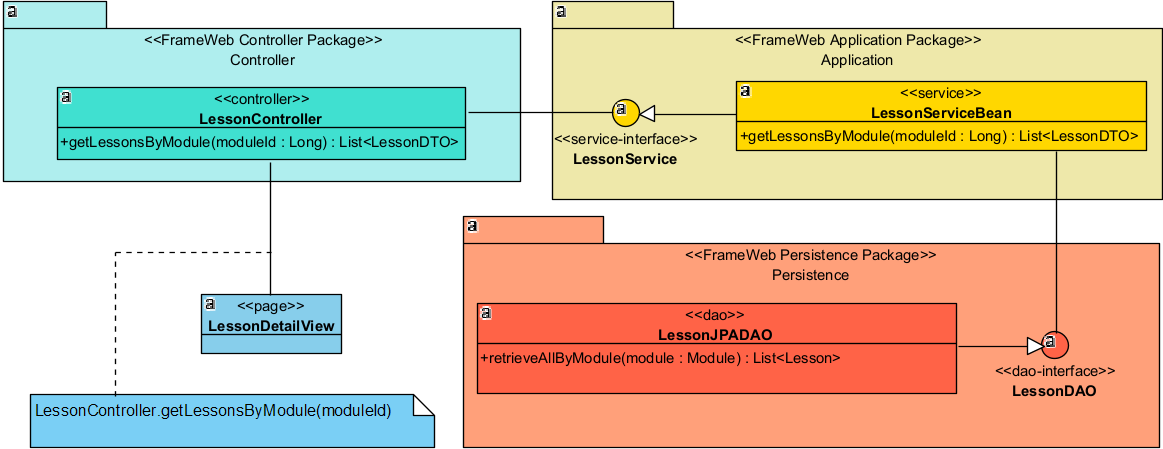
\includegraphics[width=0.8\textwidth]{figuras/marcarLicaoConcluida.png}
	\caption{Modelo de Navegação (\textsf{Marcar Lição como Concluída})}
	\label{marcarLicaoConcluida}
\end{figure}
\endgroup



%%% Páginas finais do documento: bibliografia e anexos. %%%
% Finaliza a parte no bookmark do PDF para que se inicie o bookmark na raiz e adiciona espaço de parte no sumário.
\phantompart

% Marca o início dos elementos pós-textuais.
\postextual

% Referências bibliográficas
\bibliography{bibliografia}

% Índice remissivo.
\phantompart
\printindex

% Fim do documento.
\end{document}
